\section{Carrier Generator (Lasse og Philip)}

Først opbygges kredsløbet på fumlebræt, hvor de nedenstående del-elementer testes. Når del-elementerne, er testet med succes, laves en samlet modultest for Carrier generatoren.  Efter fuldendt modultest, loddes et veroboard med de eventuelle ændringer til designet, der er foretaget.

\begin{figure}[h]
	\centering
	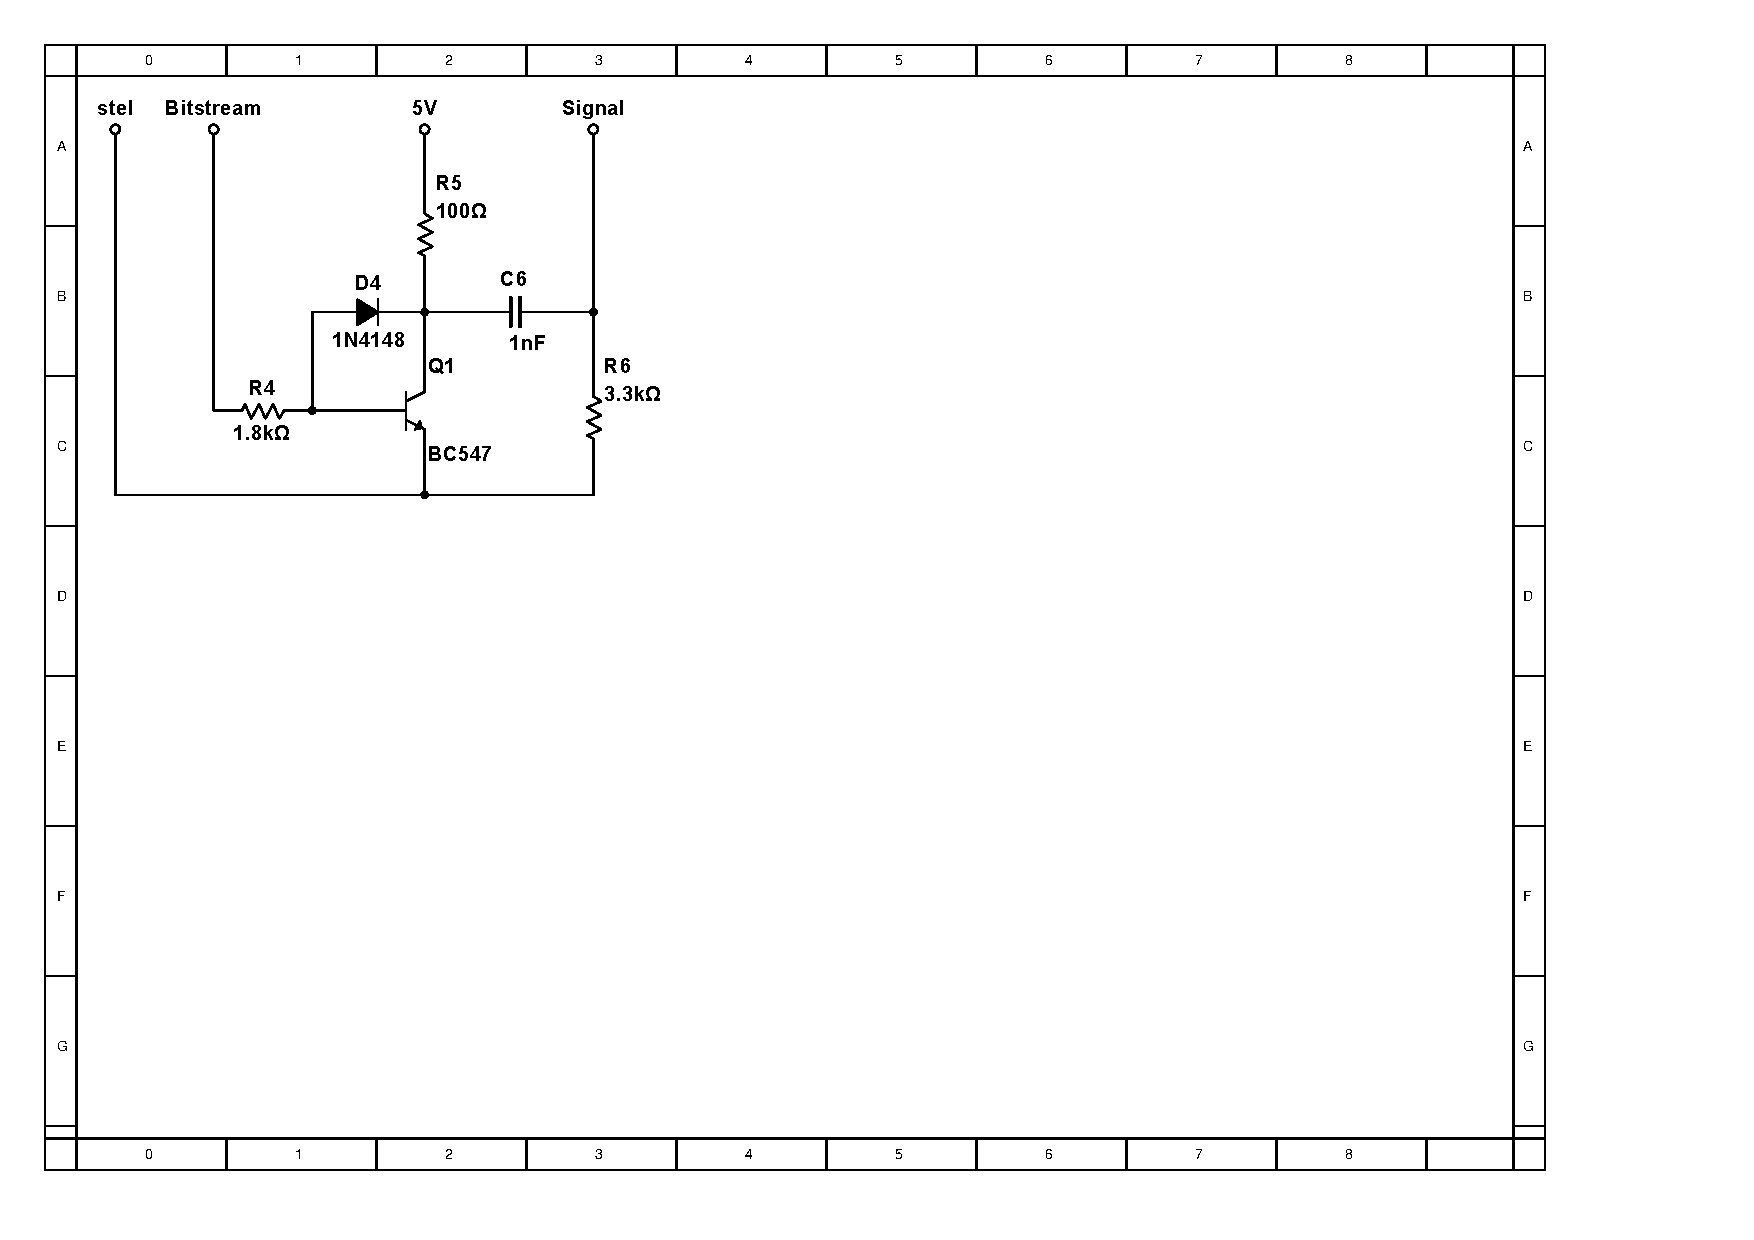
\includegraphics[scale=0.8, trim=45 355 525 45, clip=true]{../HardwareDesign/Diagrammer/CarrierGenerator.pdf}
	\caption{Carrier generator}
	\label{fig:CarrierGen}
\end{figure}

Der laves en del-test af højpasfilteret, som er består af $C_{6}$ og $R_{6}$, se figur \ref{fig:bodePlotHPFImpl}. Testen skal sikre at filteret opfører sig jf. bodeplotet i design-dokumentet på Figur \ref{fig:BodeHPF} på s. \pageref{fig:BodeHPF} i design afsnittet.

\begin{figure}[h]
	\centering
	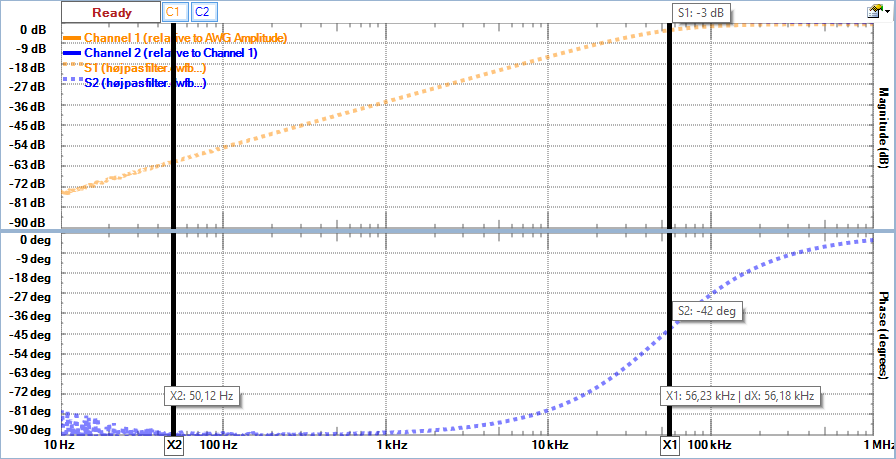
\includegraphics[width={\textwidth - 0.5 cm}, trim=0 0 0 0, clip=true]{../Implementering/billeder/BodePlotHPFLille.png}
	\caption{Analog discovery - Network Analyzer: Bodeplot af højpasfilter}
	\label{fig:bodePlotHPFImpl}
\end{figure}

Med \textit{Network Analyzer} funktionen på \textit{Analog discovery} er der konstrueret et bodeplot, der viser amplitude- og frekvenskarakteristikken for højpasfilteret. Se Figur \ref{fig:bodePlotHPFImpl}. Det ses, at knækfrekvensen ligger som forventet tæt på $50kHz$, svarene til $100\pi \cdot 10^{3} rad/s$. Ydermere kan det ses at de $50Hz$ bliver dæmpet med omkring $60dB$, hvilket er en tilstrækkelig dæmpning. Dæmpningen af $120kHz$ signalet er tæt på $0dB$. Overordnet ser det ud som forventet og som det er beskrevet i designdokumentet på side \pageref{subSecCarrierGen}.

Ved at sende et $120kHz$ firkantsignal gennem filteret, fås der et signal der viser opladning og afladning af kondensatoren.

\begin{figure}[h]
	\centering
	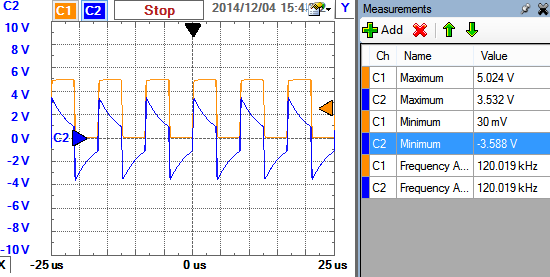
\includegraphics[width={\textwidth - 0.5 cm}, trim=0 0 0 0, clip=true]{../Implementering/billeder/filtermaaling.png}
	\caption{Måling af firkantsignal efter passering af højpasfilter.}
	\label{fig:filtermaaling}
\end{figure}

Outputtet kan ses på Figur \ref{fig:filtermaaling}. Den orange kanal viser et 120kHz firkantsignal, mens den blå viser signalet efter passage gennem højpasfilteret.\\
\\
Oprindeligt blev kredsløbet designet med en transistor ($BD139$)\cite{lib:BD139}, men det viste sig at \textit{Bitstream}, $(0V-5V 120kHz)$ firkantsignal, ikke kunne passere igennem fra transistorens kollekter til emitter. Efter en fejlsøgning kan det konkluderes, at dette skyldes en positiv opladning, når signalet var HIGH, som transistoren ikke kan nå at aflade inden næste periode. \\
Hvis transistoren skal anvendes, er det nødvendigt at fjerne den positive ladning der skabes, hurtigere end den selv kan aflade. Problemet kan løses ved at indsætte en diode ($D_{4}$)\cite{lib:1N4148} parallelt med kollekter-base benene med spærreretning mod kollektor (Baker clamp)\cite{lib:BakerClamp}. Dette vil hjælpe transistoren til at aflade den positive spænding hurtigere.\\
En anden løsning er, at skifte transistoren $BD139$ ud med en anden transistor, der har et mindre storage delay, fx $BC547$\cite{lib:BC547}. Konsekvensen heraf vil dog være at transistoren kun kan trække $100mA$ middelstrøm.\\
Der vælges en blanding af de to løsninger, således transistoren nu er en $BC547$ og der indsættes en diode parallelt med kollektor-base benene.

\begin{figure}[h]
	\centering
	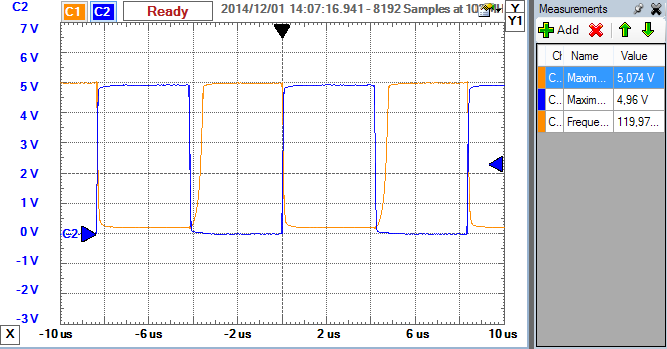
\includegraphics[width={\textwidth - 0.5 cm}, trim=0 0 0 0, clip=true]{../Implementering/billeder/TransistorImpl.png}
	\caption{Analog discovery - Oscilloskop: Transistor-kredsløb}
	\label{fig:TransistorImpl}
\end{figure}

På figur \ref{fig:TransistorImpl} ses en oscilloskop-måling af transistor-kredsløbet. Her ses at udgangen \textit{Signal} (den orange), er inverteret i forhold til indgangen \textit{Bitstream} (den blå). Det kan ligeledes ses at der er en lille opladning- og afladningstid på udgangen, der skyldes opladningen af transistoren. Dette har ingen betydning i forhold til anvendelsen af signalet.\\

\newpage
En samlet modultest af Carrier generator udføres med et oscilloskop på udgangen af carrier generatoren (\textit{Signal}).\\

\begin{figure}[h]
	\centering
	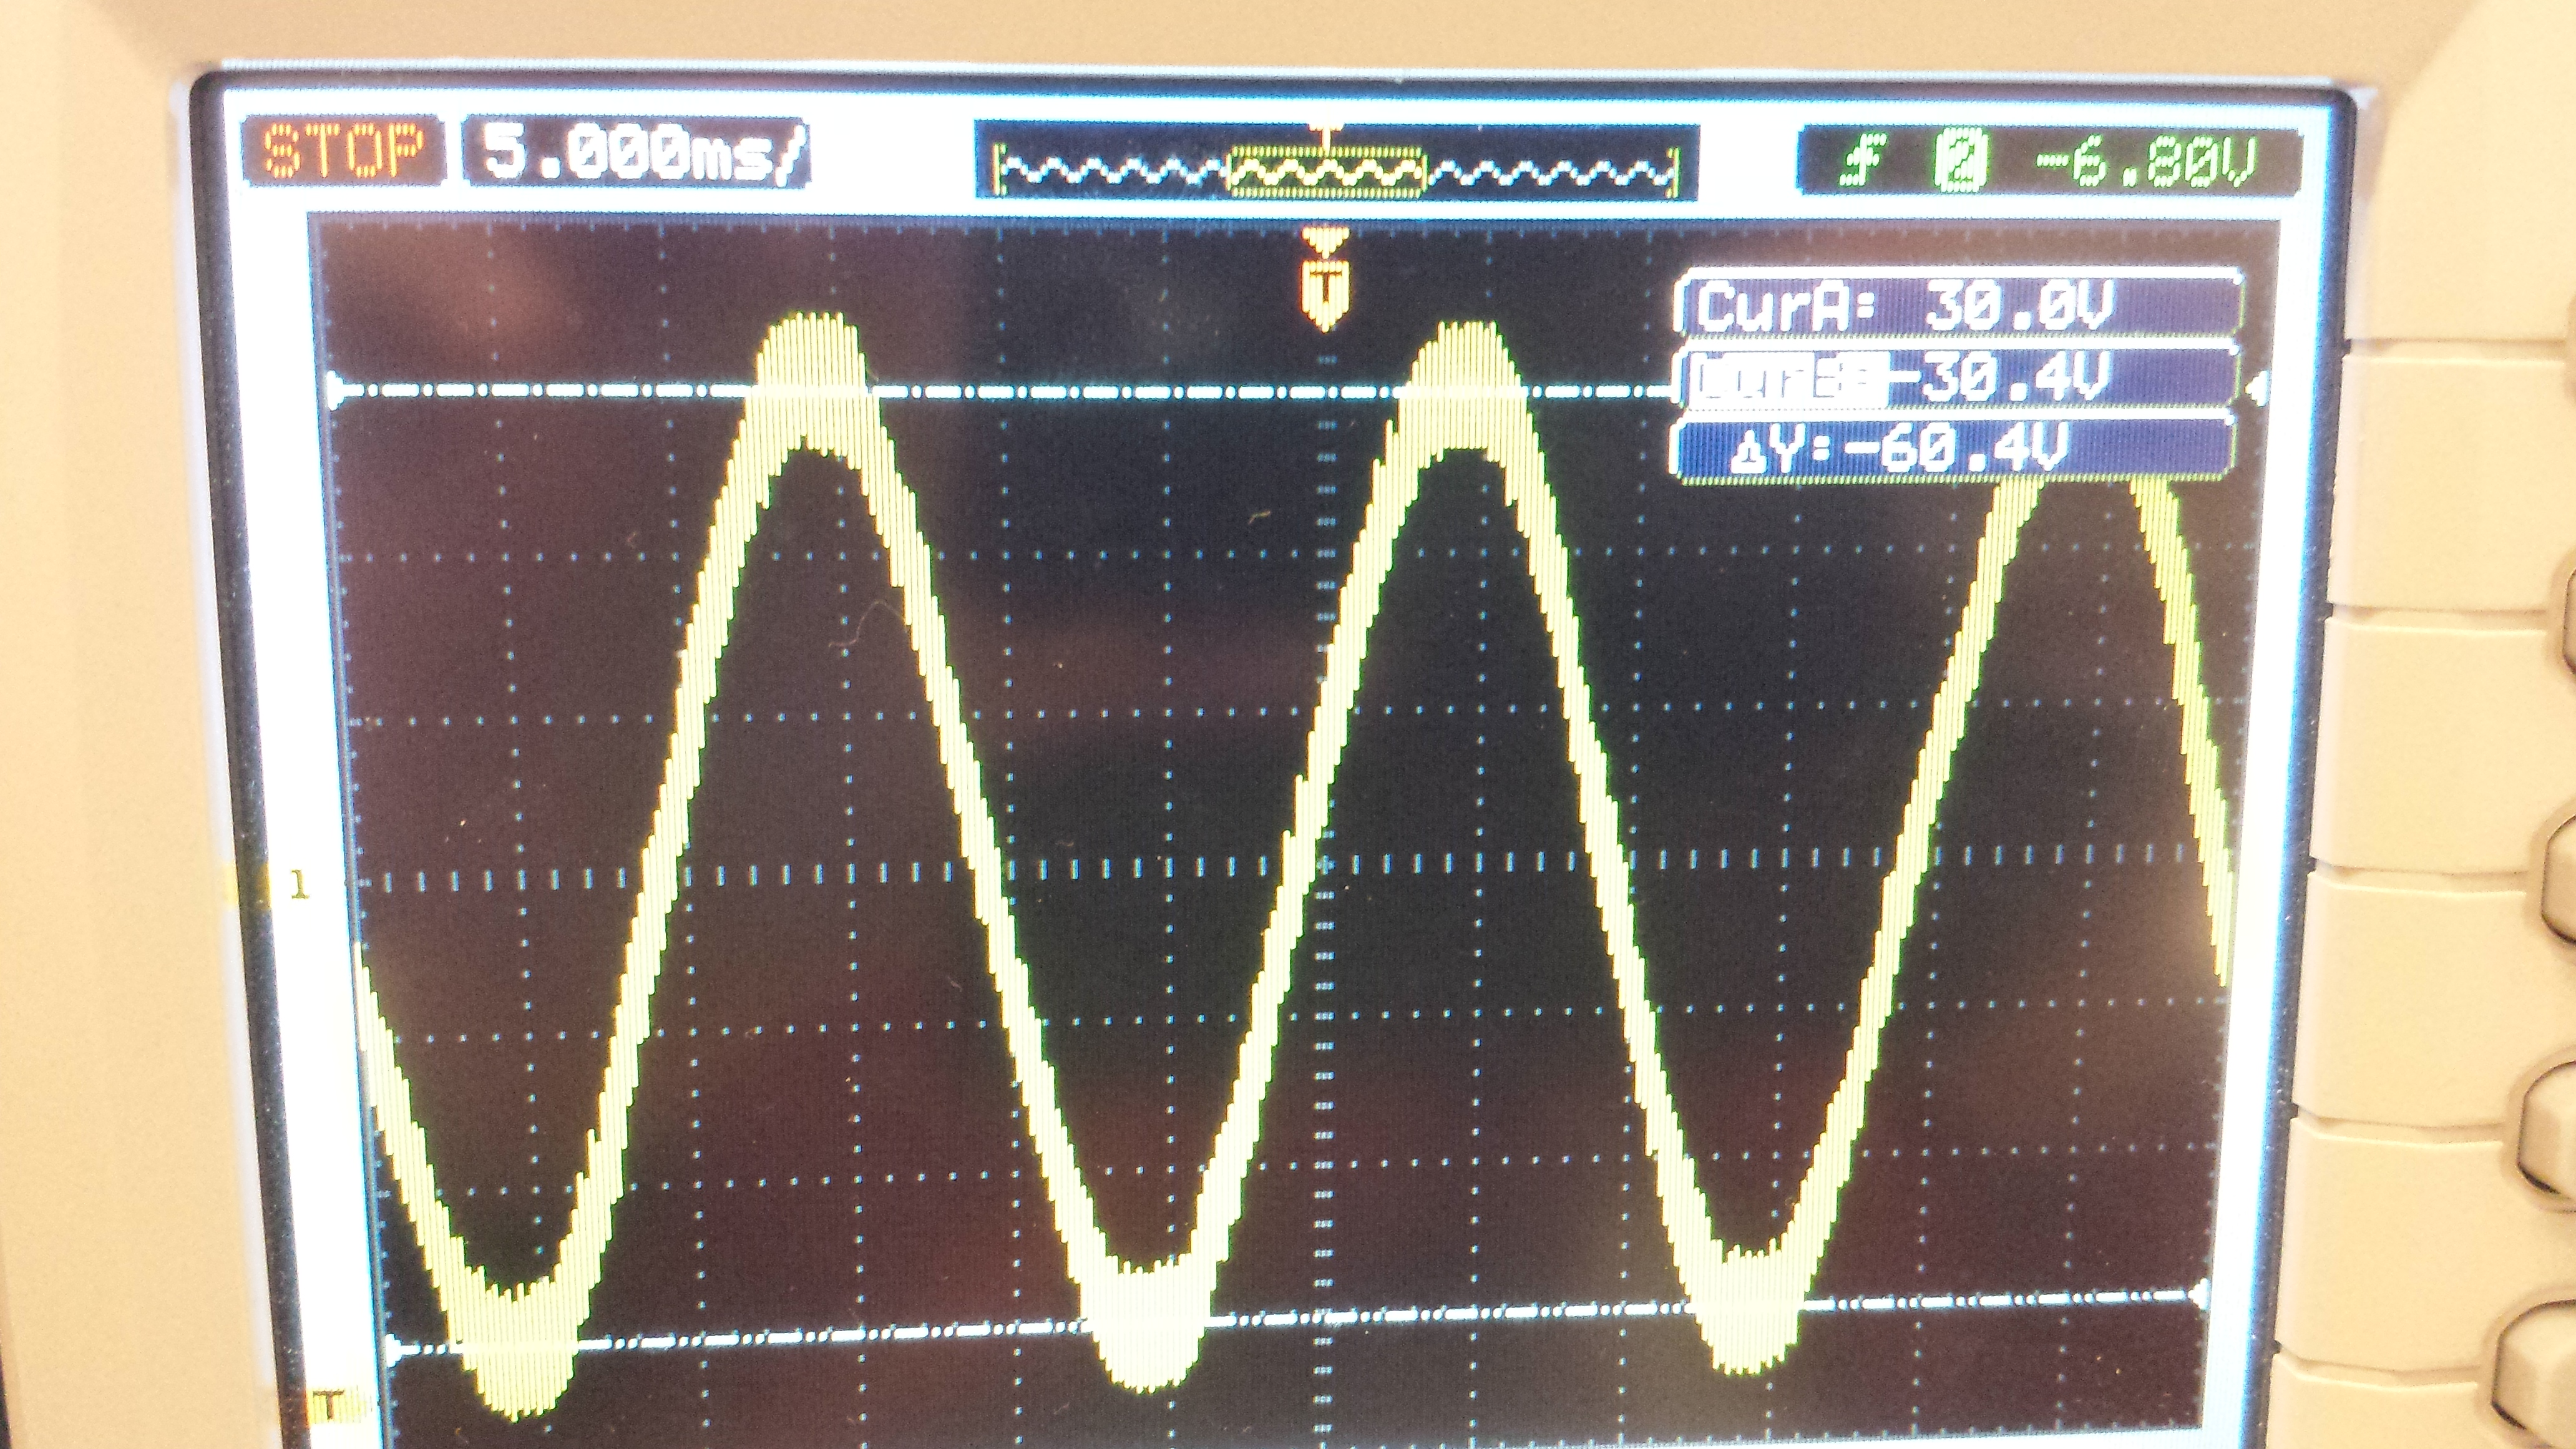
\includegraphics[width={\textwidth - 1 cm}, trim=0 0 0 0, clip=true]{../Implementering/billeder/CGImpl1.jpg}
	\caption{Oscilloskop: Carrier generator modultest }
	\label{fig:CGImpl1}
\end{figure}

\begin{figure}[h]
	\centering
	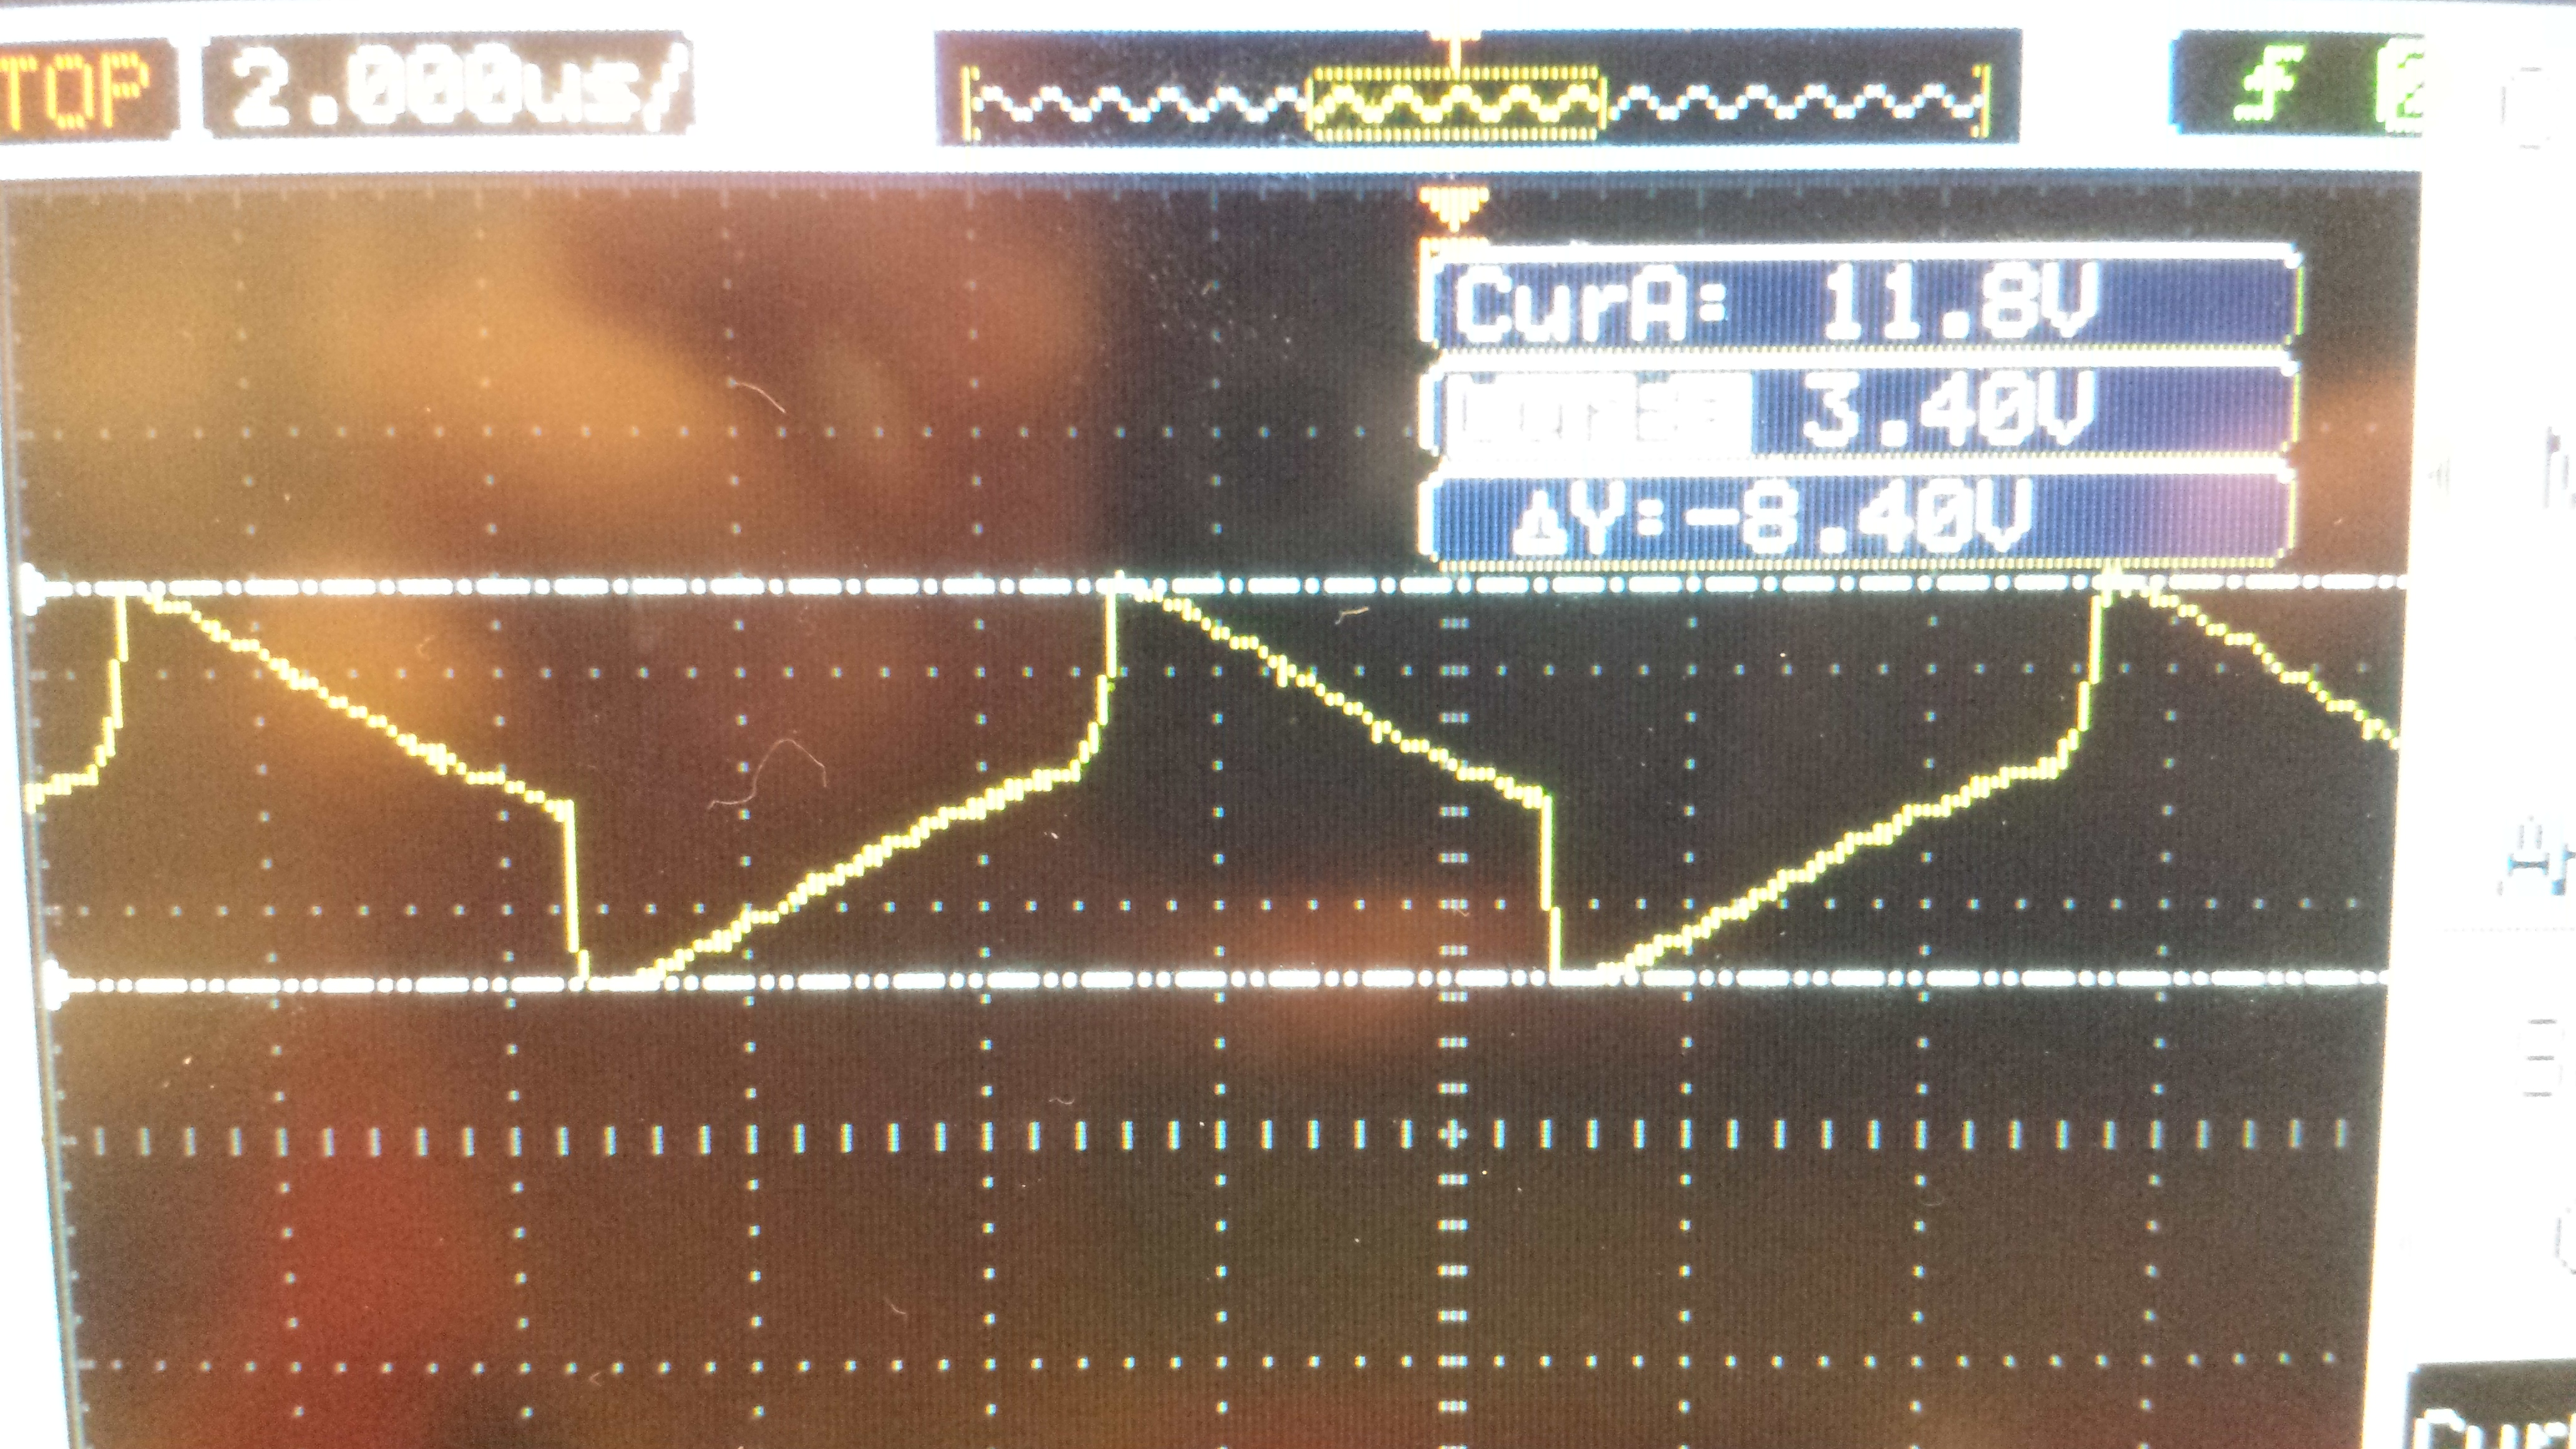
\includegraphics[width={\textwidth - 1 cm}, trim=0 0 0 0, clip=true]{../Implementering/billeder/CGImpl2.jpg}
	\caption{Oscilloskop: Carrier generator modultest zoom }
	\label{fig:CGImpl2}
\end{figure}

\newpage

Figur \ref{fig:CGImpl2} viser samme signal som figur \ref{fig:CGImpl1}. Der er blot zoomet ind så der kun er $2us$ mod $5ms$ pr. streg på tidsaksen. Testen viser at der bliver påtvunget et $120kHz$ signal på udgangen \textit{Signal}, der i forvejen indeholder en $18VAC - 50Hz$ frekvens.\\
Det bemærkes at signalet har en peak to peak spænding på $3.4V$, hvilket skyldes spændingsdeling i kredsløbet.